%!TEX root=protocol.tex	% Optional

\section{Umsetzung}
Die Umsetzung wurde mit diffsync gemacht.

\subsection{Voraussetzungen}

Für das Testen der Umsetzung ist folgendes Vorausgesetzt:
\begin{itemize}
	\item Node.js 8 LTS
\end{itemize}


% diffsync
\subsection{Synchronisationsalgorithmus}
Die Datensynchronisation in Echtzeit bei verteilten Systemen ist eine Herausforderung, da die Daten von verschiedenen Usern immer konsistent gehalten werden müssen. Für die Echtzeit muss die Synchronisation sehr häufig durchgeführt werden. Es gibt verschiedene Methoden und Algorithmen, um dies zu erzielen.

\subsubsection{Herausforderungen}

Der Synchronisationsprozess muss möglichst oft durchgeführt werden. Benötigt der Client zu viel Zeit, um mit dem Server zu synchronisieren, ist die Wahrscheinlichkeit für einen Zusammenführungskonflikt viel höher. Au"serdem muss die Version des Servers und die des Clients konsistent bleiben. In verteilten Systemen ist dies nicht möglich, au"ser der Datenbestand wird blockiert, bis der andere Client die Änderung durchgeführt hat. In NoSQL-Systemen wird mit schlussendlicher Konsistenz gearbeitet. Dieses Modell verlangt nicht, dass der Datenbestand sofort mit der Gegenseite übereinstimmt, muss jedoch möglichst schnell einen konsistenten Zustand erreichen. \cite{websocket-consistency-tanenbaum}

Dennoch kann es zu Konflikten kommen. Wenn mehrere User an derselben Stelle eines Dokuments eine Änderungen durchführen, kommt es zu Problemen bei der Zusammenführung. Bei Synchronisationsprozessen, die nicht in Echtzeit durchgeführt werden, wird der User um eine manuelle Zusammenführung gebeten. In einem System, in der die Echtzeit wichtig und die Zusammenführung sehr häufig durchgeführt wird, ist eine manuelle Zusammenführung nicht möglich.

Auch die Möglichkeit eines Paketverlustes muss beachtet werden, wenn in einem verteilten System die Verbindung nicht zuverlässig ist. Der Client oder der Server hat keine Möglichkeit zu erkennen, ob die Gegenseite dessen Änderungen eingefügt hat. Im schlimmsten Fall arbeiten der Client und der Server mit unterschiedlichen Versionen, und dadurch ist die Konsistenz nicht gewährleistet. \cite{websocket-consistency-tanenbaum}

Es existieren verschiedene etablierte Synchronisationsmethoden, welche jedoch nicht für jede Situation geeignet sind. Abhängig von der Methode wird entweder die Konsistenz oder die Echtzeit priorisiert.

\subsubsection{Sperrbasiert/Wechselweise}
Bei dieser Methode wird nur ein User für das Editieren eines Dokuments zugelassen. Während dieser User den vollen Schreibzugriff hat, müssen andere warten, bis der User seine Änderungen durchgeführt hat. Die anderen User haben während der Dauer des Editierungsvorgangs nur Lesezugriff. \cite{websocket-differential}

Der Nachteil dieser Methode ist, dass nur ein User das Dokument editieren kann, und daher die Methode für kollaboratives Editieren nicht geeignet ist.

\subsubsection{Änderungsbasierte Synchronisation}
Bei der änderungsbasierten Synchronisation wird dem jeweiligen anderen Client der Änderungsbefehl mitgeteilt. Diese Methode ist sehr effizient, da nur sehr wenig Information übertragen werden muss. Jedoch müssen alle Änderungen beachtet werden. Darunter fallen Befehle wie einfache Editierungen, aber auch Kopieren, Einfügen, Ersetzen und die Autokorrektur.

Arbeiten mehrere User an einem Dokument, kann es zu Konflikten kommen, wenn gleichzeitig Änderungen durchgeführt werden. Wenn Client A an einer Textpassage eine Änderung durchführt und Client B an der gleichen Textpassage eine andere Änderung durchführt, dann werden diese an den Server geschickt. Der Server sendet dann die jeweiligen Änderungsbefehle an den jeweiligen anderen User.

\makefig{images/sync/ot-problem.png}
{width=0.65\textwidth}
{Probleme mit änderungsbasierter Synchronisation \cite{websocket-diffsync-presentation}}
{websocket-ot-problem}

Sollte es zu so einem Fall kommen, dann arbeiten die verschiedenen Clients mit unterschiedlichen Versionen des Dokuments. Die Clients haben keine Möglichkeit, diese Inkonsistenz zu erkennen.

Weiterhin kann es zu einer Inkonsistenz kommen, wenn Änderungsbefehle über das Netzwerk verloren gehen. Der Client A nimmt an, dass die Änderungen bei Client B durchgeführt wurden, obwohl dies nicht der Fall ist. Auch hier kann die Inkonsistenz nicht erkannt werden.

\paragraph{Dreiweg-Zusammenführung}~\\
Die Dreiweg-Zusammenführung ist sehr bekannt, da sie in Versionierungssoftware wie Git oder SVN eingesetzt wird. Bei der Dreiweg-Zusammenführung ist eine Basisversion vorhanden, von der jeder Client ausgeht. Machen zwei Clients gleichzeitig eine Änderung, kann dies durch die Dreiweg-Zusammenführung gelöst werden.

\makefig{images/sync/diagrams/2-3way.png}
{scale=0.4}
{Dreiweg-Zusammenführung}
{websocket-3way}

% TODO: Cite Icon Author???

Die Client-Version und die Server-Version gehen von einer Basis-Version aus. Diese wird benötigt, um von beiden Seiten (Server und Client) die Änderungen zusammenzuführen.

Die Dreiweg-Zusammenführung bietet die Möglichkeit, dass gleichzeitig mehrere Personen an einem Dokument arbeiten können. Jedoch dürfen während der Phase der Zusammenführung keine Änderungen vorgenommen werden, da die Basis-Version immer gleich sein muss. Daher ist diese Methode nicht für Echtzeit-Anwendungen geeignet.

\newpage
\paragraph{Differentialsynchronisation}~\\
Die Differentialsynchronisation ist ein Synchronisationsalgorithmus, der von Neil Fraser entwickelt wurde. \cite{websocket-differential} Bei der Differentialsynchronisation arbeiten der Server und der Client jeweils mit einem Schattendokument. Dabei besitzt der Server \textbf{pro User} ein eigenes Schattendokument. 

\makefig{images/sync/diff-dual-shadow.png}
{width=0.6\textwidth}
{Differentialsynchronisation mit doppeltem Schattendokument \cite{websocket-differential}}
{websocket-dual-shadow}

Nach jeder Änderung wird versucht, das Dokument mit dem Server zu synchronisieren.

\begin{enumerate}
	\item Der veränderte Text des Clients wird mit dem Schattendokument verglichen.
	\item Die Liste an Änderungen wird gesammelt.
	\item Der veränderte Text wird zum Schattendokument.
	\item Die Veränderungen vom Client werden mit dem Schattendokument auf der Server-Seite zusammengefügt.
	\item Das zusammengeführte Dokument ergibt das neue Schattendokument.
	\item Die Veränderungen vom Client werden mit dem Dokument des Servers zusammengeführt.
	\item Das zusammengeführte Dokument ergibt das neue Server-Dokument.
\end{enumerate}

Es darf immer nur ein Netzwerk-Paket versendet werden. Das hei"st, dass, wenn der Client ein Paket sendet, der Server keines senden darf, bis dieses Paket angekommen ist. Im obigen Modell (Abbildung \ref{websocket-dual-shadow}) ist es jedoch nicht möglich, dies zu erkennen. Daher müssen sich der Client und der Server mit dem Senden und Empfangen abwechseln, damit es nicht zu Konflikten kommt.

Der gleiche Prozess kann auch in die andere Richtung durchgeführt werden. Es ist essentiell, dass das Schattendokument der Client-Seite und das auf der Server-Seite gleich sind. Dabei können Prüfsummen helfen sicherzustellen, dass die Dokumente übereinstimmen. Die Schattendokumente sind die Basis für richtige Patches. Wenn nun ein Paket verloren geht, dann hat der Server keine Möglichkeit, die Änderungen anzunehmen. Daraus folgt, dass die Schattendokumente auf der Client- und Server-Seite nicht gleich sind. Der Client würde bei einer weiteren Änderung mit einem falschen Schattendokument arbeiten.

\paragraph{Differentialsynchronisation mit garantierter Übermittlung}~\\
Dieses Modell basiert auf der Differentialsynchronisation mit dem Zusatz von Versionsnummern und einem Backup-System.

\makefig{images/sync/diff3a.png}
{width=0.8\linewidth}
{Differentialsynchronisation mit garantierter Übermittlung \cite{websocket-differential}}
{websocket-dual-shadow-with-guaranteed-delivery}

\begin{enumerate}
	\item Der veränderte Text des Clients wird mit dem Schattendokument verglichen.
	\item Änderungen werden in einer Liste gesammelt. Es handelt sich hierbei um eine Liste von Änderungen mit den jeweiligen Versionsnummern.
	\item Der veränderte Text wird zum Schattendokument. Die Versionsnummer des Clients erhöht sich. Nach diesem Schritt werden die Veränderungen an den Server versendet. Dabei hat jede Veränderung ihre eigene Versionsnummer und eine gemeinsame Server-Versionsnummer. Die Liste an Änderungen wird erst dann gelöscht, wenn der Server dies auch bestätigt.
	\item Die Server-Versionsnummer wird verglichen. Falls die Server-Versionsnummer vom Client älter sein sollte, wird das Backup-Schattendokument geladen.
	\item Die Veränderungen vom Client werden mit dem Schattendokument auf der Server-Seite zusammengefügt.
	\item Das zusammengeführte Dokument ergibt das neue Schattendokument. Die Client-\\Versionsnummer wird auf den neuesten Stand gesetzt.
	\item Das momentane Schattendokument überschreibt das Backup-Schattendokument.
	\item Die Veränderungen vom Client werden mit dem Dokument des Servers zusammengeführt.
	\item Das zusammengeführte Dokument ergibt das neue Server-Dokument.
\end{enumerate}

\newpage
Auch hier kann der gleiche Prozess in der anderen Richtung durchgeführt werden, mit dem Unterschied, dass auf der Client-Seite kein Backup-Schattendokument existiert. Durch den Einsatz eines Backup-Schattendokuments können mögliche Probleme behandelt werden:

\begin{itemize}
	\item \textbf{Doppeltes Paket:} In diesem Fall werden die Änderungen zweimal versendet. Die Versionsnummer ist dabei gleich. Beim ersten Mal werden diese Änderungen vom Server bearbeitet. Beim zweiten Mal erkennt der Server jedoch, dass seine Client-Versionsnummer höher ist. Die Änderungen werden ignoriert.
	\item \textbf{Verlust eines Client-Pakets:} In diesem Fall geht beim ersten Versenden das Netzwerk-Paket verloren, beim zweiten Mal jedoch nicht. Da die Liste an Änderungen erst bei einer Antwort des Servers gelöscht wird, kann der Client nach einer kurzen Zeit diese Liste wieder versenden. In dieser Zeit hat der Client auch die Möglichkeit, weitere Änderungen durchzuführen.
	\item \textbf{Verlust eines Server-Pakets:} In diesem Fall hat der Client seine Antwort nie bekommen. Der Client nimmt an, dass sein Client-Paket verloren ging. Er sendet deswegen nochmal ein Client-Paket. Der Server merkt, dass die Server-Versionsnummern nicht übereinstimmen. Daraufhin lädt der Server die alte Version vom Backup-Schattendokument und beginnt wieder von dieser Version aus seine Änderungen durchzuführen.
\end{itemize}

Wie auch bei der Dreiweg-Zusammenführung kann es in diesem Modell zu unlösbaren Zusammenführungskonflikten kommen. Im Unterschied zur Dreiweg-Zusammenführung verläuft die Differentialsynchronisation in einer Umgebung, in der die Echtzeit wichtig ist. Es besteht hier keine Möglichkeit, dass eine Person diese Konflikte manuell lösen kann. Falls es zu einem unlösbaren Zusammenführungskonflikt kommen würde, wird der Client gezwungen, auf den Stand des Servers zurückzukehren. Da die Synchronisation sehr häufig geschieht, sind diese Verluste minimal.


% \subsection{Die Synchronisation}
% Für den Synchronisationsalgorithmus wurde die Differentialsynchronisation ausgewählt, da es sowohl auf die Konsistenz als auch auf die Effizient achtet. Dieser Algorithmus wurde von Neil Fraser entwickelt. \cite{websocket-differential} ''diffsync`` ist eine Implementierung des Algorithmus für die Node.js-Umgebung und kann direkt mit Socket.io verwendet werden.

% Es existieren auch andere Synchronisationsalgorithmen, welche aber nicht für Echtzeit-Kommunikation geeignet sind. So bietet der Three-Way-Merge eine Methode der Zusammenführung, welche auch bei git verwendet wird.

\paragraph{Skalierung und Replikation}
Die einfachste Möglichkeit, dieses System zu skalieren, ist es, die Anwendung auf verschiedenen Rechnern zu verteilen, die jeweils für eine bestimmte Anzahl an Dokumenten zuständig sind. 

Sollte jedoch eine Skalierung auf ein einzelnes Dokument benötigt werden, dann teilen sich die jeweiligen Server die Benutzer. Die Differentialsynchronisation kann auch zwischen Server und Server angewendet werden. 


\makefig{images/server2.png}
{width=0.8\linewidth}
{Differentialsynchronisation mit mehr als zwei Servern \cite{websocket-differential}}
{websocket-dual-shadow-2s2}

% \begin{figure}[!h]
% 	\begin{center}
% 		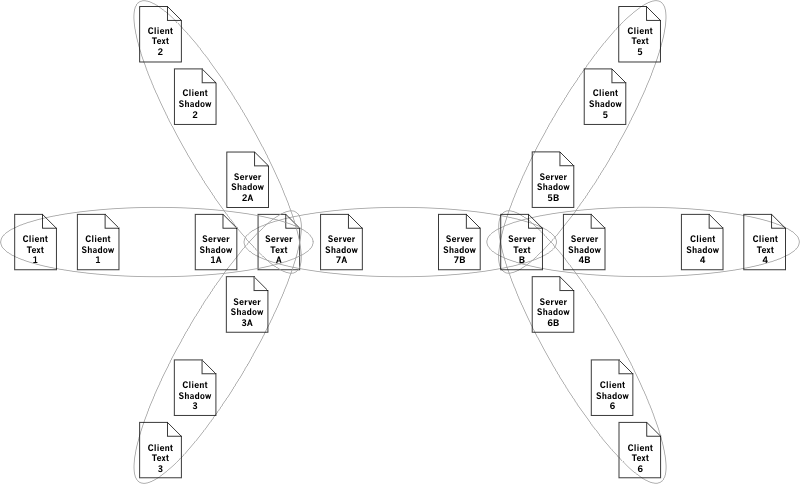
\includegraphics[width=0.8\linewidth]{images/server2.png}
% 		\caption{Differentialsynchronisation mit mehr als zwei Servern \cite{websocket-differential}}
% 		\label{websocket-dual-shadow-2s2}
% 	\end{center}
% \end{figure}

\subsection{diffsync}
Diffsync ist eine leightweight Library für die Differentialsynchronisation. Es bietet eine Adapter-Schnittstelle, welche für das jeweilige gewünschte Framework implementiert werden kann. Die Schnittstelle besteht aus den Methoden \codein{js}{getData()} und \codein{js}{storeData()}.

\subsection{Die Replikation}
Da diffsync unabhängig vom Datenbankmanagementsystem ist, kann jedes verwendet werden. Couchbase ist eine NoSQL-Datenbank, welche Replikationsmöglichkeiten bietet. So kann diffsync mit Couchbase integriert werden, wenn der Adapter implementiert wird.

\subsection{Server}
Der Server besteht lediglich aus der diffsync-Library und Socket.io welche auf Port 3000 lauscht. Diffsync kümmert sich um die Synchronisierung nach dem Differentialalgorithmus. Dank Socket.io ist auch eine automatische Wiederverbindung möglich.

\subsection{Client}
Der Client besteht aus der index.html und der Javascript-Datei index.js welches in ES6 geschrieben wurde und mit webpack in einer bundle.js transpiliert wird.

\subsubsection{Funktionsweise}

Die Web-Applikation besteht aus mehrere Funktionalitäten. Dies Umfasst die CRUD-Operationen für die Applikation.

\paragraph{DOM-Modifikation}
Nach jeder Veränderung des data-Objekts wird das ganze DOM-Model neu gebildet. Dies bedeutet, dass alle DOM-Elemente gelöscht und neu hinzugefügt werden. Damit wird garantiert, dass das DOM-Model auch die Daten im data-Objekt repräsentiert. Außerdem wird ein sync-Befehl ausgeführt. Damit erhalten alle anderen verbundenen Clients die Daten und deren View wird auch aktualisiert.

\paragraph{Hinzufügen von Daten}
Wenn nun neue Daten hinzugefügt werden, dann wird das \codein{js}{data}-Objekt verändert. Die View wird aktualisiert und die Synchronisation wird ausgeführt.

\paragraph{Löschen von Daten}
Ein Datensatz kann mithilfe des ``Löschen''-Buttons gelöscht werden. Der jeweilige Datensatz wird mithilfe der Position in der Liste identifiziert.

\paragraph{Aktualisieren von Daten}
Datensätze können aktualisiert werden, in dem man auf den ``Editieren''-Button klickt. Der Datensatz wird dann gelöscht, und die Daten werden in den Editierungsboxen kopiert. Danach können die Daten wieder hinzugefügt werden. 


\subsection{Ausführung}

\subsubsection{Server}
Um den Server zu starten müssen folgende Schritte befolgt werden:
\begin{itemize}
	\item In der Ordner des Server eintreten: \codein{text}{cd server}
	\item \codein{text}{npm install} ausführen, damit alle Abhängigkeiten installiert werden
	\item \codein{text}{npm start} ausführen, um den Websocket-Server zu starten.
\end{itemize}

\subsubsection{Client}
Um den Client zu testen müssen folgende Schritte befolgt werden:
\begin{itemize}
	\item In der Ordner des Clients eintreten: \codein{text}{cd client}
	\item \codein{text}{npm install} ausführen, damit alle Abhängigkeiten installiert werden
	\item \codein{text}{npm start} ausführen damit der Client von webpack kompiliert wird.
	\item \codein{text}{npm run server} ausführen damit ein HTTP-Server auf 8080 gestartet wird, welche die Client-HTML-Datei ausgibt.
\end{itemize}





